% !TEX encoding = UTF-8 Unicode
\documentclass[conference]{IEEEtran}
\usepackage{amsmath} 
\usepackage{url}
\usepackage{subfigure}
\usepackage{graphicx,epsfig}
\hyphenation{op-tical net-works semi-conduc-tor}

                                         % Activate to display a given date or no date

\begin{document}

\title{Evolutionary Art using Processing}
% author names and affiliations
% use a multiple column layout for up to three different
% affiliations
\author{\IEEEauthorblockN{Author 1}
\IEEEauthorblockA{Affiliation 1\\
University of Granada\\
Email:}
\and
\IEEEauthorblockN{Author 2}
\IEEEauthorblockA{Affiliation 2\\
University of Granada\\
Email:}
\and
\IEEEauthorblockN{Author 3}
\IEEEauthorblockA{Affiliation 3\\
University of Granada\\
Email:}
}

\maketitle

\begin{abstract}
This paper shows how the Processing framework can be used to generate Evolutionary Art. Processing is a framework designed for visual designers and artists that is starting to have great pressence in the interactive and visual art field. It includes several modules for image creation, manipulation and analysis. This framework has been used to create an Evolutionary Algorithm that generates images comparing the histograms of a test image. Three different fitness functions have been used: the differences of the RGB histogram, the HSV histogram and an average of both. Results shows that the latter increases the similirities of the RGB and HSV with respecting to using them separately.
\end{abstract}

\section{Introduction}\label{intro}
Evolutionary art blah, blah, blah, ...

The main goal of this paper is ... We show ...

This paper is organized as follows: in Section \ref{sec:soa}, a brief review on Evolutionary Art is presented. Processing and image information are described next (Section \ref{sec:processing}). The experimental setup and results are presented in Sections \ref{sec:setup} and \ref{sec:results}, respectively. Finally, the conclusions and future work can be found in Section \ref{conclusions}.

\section{State of the art}
\label{sec:soa}

Computational Aesthetics ``is the research of computational methods that can make applicable aesthetics decisions in a similar fashion as humans can'' \cite{COMPAESTH}. In the field of computational aesthetics, evolutionary systems can play an important role, enabling the evolution of aesthetically pleasing or innovative structures \cite{dipaola2009incorporating}.


Representation of the art in Evolutionary Art can be one of the methods in the following classification:
\begin{itemize}
	\item Symbolic expression. The genotype is a tree of expressions and the phenotype consists in the image produced  by the evaluation of the tree.
	\item Grammars. A shape grammar is used as a formal description of the image.
	\item Using existing images as a source. 
	\item Others, such as fractals or cellular automata.
\end{itemize}

One of the main challenges in Evolutionary Art is how to measure aesthetic value of an piece of evolutive art.

Two modes of aesthetics measures are defined by \cite{galanter2012computational}: 
\begin{enumerate}
\item ``{\em Aesthetics evaluations are expected to simulate, predict or cater to humans notions of beauty and taste.}'' This will be the definition used in this paper. 
\item ``{\em Is an aspect of meta-aesthetic exploration and usually involves aesthetic standards created by software agents in artificial worlds.}''
\end{enumerate}

According to Galanter \cite{galanter2012computational}, computational aesthetics measures can be classified in the following categories:
\begin{itemize}
	\item Based on Formulaic and Geometric Theories. The aesthetics of a piece of art are evaluated using a formula o principle (e.g., pythagorean proportions).
	\item Based in Design Principles. Like the rule of thirds or theory of color (e.g., using opposite colors).
	\item Based in Neural Networks and Connective Models. 
	\item Complexity Based Models. 
	\item Based in Evolutionary Systems:
		\begin{itemize}
			\item Interactive Evolutionary Computation. The fitness of the individuals is determined by human agents.
			\item Performance based goals. Certain properties of the art piece are evaluated and optimized based in performance measures (e.g., usable surface in a furniture design generator).  
			\item Error relative to Exemplars. The individual fitness is measured using a real-world example (e.g., a photography).
			\item Complexity measures. This type of measures is based in the idea the complexity is directly related to aesthetics and follows the path firstly stablished by Birkhoff \cite{birkhoff2003aesthetic}.
			\item Multi-objective. Given the multidimensional nature of aesthetics judgement, multi-objective EAs are a clear option in order to deal with this multidimensionality.
			\item Extensions to EA (such as, coevolution, agent swarm behavior, etc.).
		\end{itemize}
\end{itemize}

A brief classification of the aesthetic measures found in a short review can be fount in Table~\ref{table_class}.

%PAPERS LEÍDOS
%En \cite{li2012investigating}, Li et al. proponen las siguiente métricas para el aprendizaje estético:
%\begin{itemize}
%	\item Color ingredient.
%	\item Image complexity.
%	\item Image order.
%	\item MC metric.
%	\item BL Metric.
%\end{itemize}
%
%En \cite{den2010using}, presenta una comparación de tres métricas estéticas:
%\begin{itemize}
%	\item Benford Law.
%	\item Global Contrast Factor.
%	\item Information Theory.
%\end{itemize}
%
%En \cite{den2010comparing}, presenta una comparación de cuatro métricas estéticas:
%\begin{itemize}
%	\item Machado and Cardoso.
%	\item Ross and Ralph.
%	\item Fractal Dimension.
%	\item A weighted sum of the above mentioned metrics.
%\end{itemize}
%
%En \cite{den2011evolving} se presenta una aproximación multi-objetivo para arte evolutivo. Las tres funciones de fitness utilizadas son:
%\begin{itemize}
%	\item Benford Law.
%	\item Global Contrast Factor.
%	\item Ross and Ralph (bell curve).
%\end{itemize}
%
%En \cite{den2012evolving} se presenta un AE para crear arte evolutiva a partir de imágenes vectorizadas. La función de fitness utilizada es la diferencia de tono entre  distintas regiones de la imagen a distintas resoluciones.
%
%En \cite{dipaola2009incorporating} they present an automatic fitness function specific to portrait painting based in four scores:
%\begin{itemize}
%	\item Resemblance.
%	\item Composition (face vs background).
%	\item Tonality.
%	\item Color.
%\end{itemize}

%\rowcolors{2}{gray!25}{white}
\begin{table*}[!t] 
%\renewcommand{\arraystretch}{1.3} 
\caption{Classification of the aesthetic measures used in a brief review of the literature on evolutive art.} 
\label{table_class} 
\centering
\begin{tabular}{|l|l|}
\hline
Type & Aesthetic Measure \\ \hline
Formulaic and Geometric Theories & Fractal dimension \cite{den2010comparing}, Image order \cite{li2012investigating}, Benford Law \cite{del2005benford}\\ \hline
Based in Design Principles &  Color contrast (hue) \cite{den2012evolving},  Color ingredient \cite{li2012investigating}, Composition, tonality and color \cite{dipaola2009incorporating}.\\ \hline
Interactive Evolutionary Computation & The electric sheep project \cite{draves2006electric} \\ \hline
Error relative to Exemplars &  Resemblance score \cite{dipaola2009incorporating}, pixel comparation \cite{aguilar2008robotic}\\ \hline
Performance based goals & Evolving virtual creatures \cite{sims1994evolving} \\\hline
Complexity measures & Image complexity \cite{li2012investigating}, Machado and Cardoso aesthetic measure \cite{machado1998computing}\\ \hline
\end{tabular}
\end{table*}

\section{Processing and image metrics}
\label{sec:processing}
In this section we will describe Processing \footnote{\url{http://www.processing.org/}}. Processing \cite{PROCESSING} is a framework formed by a simple programming language and an integrated development environment (IDE) mainly focused to electronic and visual artists, designers, musicians, etc.

Processing has the next advantages:

\begin{itemize}
\item Processing was created for artists, rather than programmers. So, it allows very complex drawings and interactive applications with few lines of code. For example, Figure \ref{fig:subide} shows the sketch (in the IDE) necessary to create the Figure \ref{fig:subsketch}.
\item It is an Open Source software, and can work with the community in its development.
\item It is based in OpenGL, obtaining a good 3D acceleration.
\item Includes more than 100 libraries for video, sound, phisycs, computer vision, networking, etc.
\item Easy integration with Java, HTML5 and Android.
\item Finally, it is fairly light when installed.
\end{itemize}

\begin{figure*}[ht]
\centering

\subfigure[Processing IDE]{
   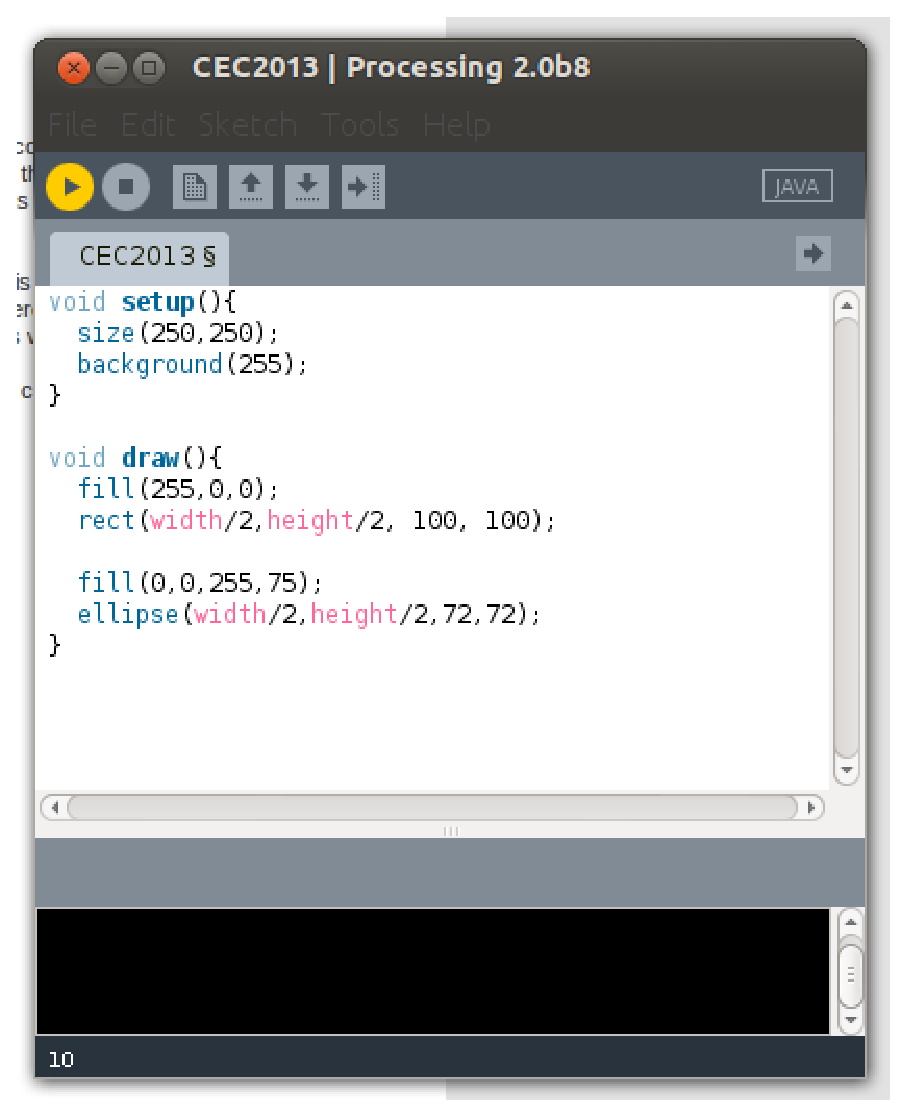
\includegraphics[scale =0.55] {images/Processing.eps}
   \label{fig:subide}
 }
\subfigure[Runtime of the code.]{
   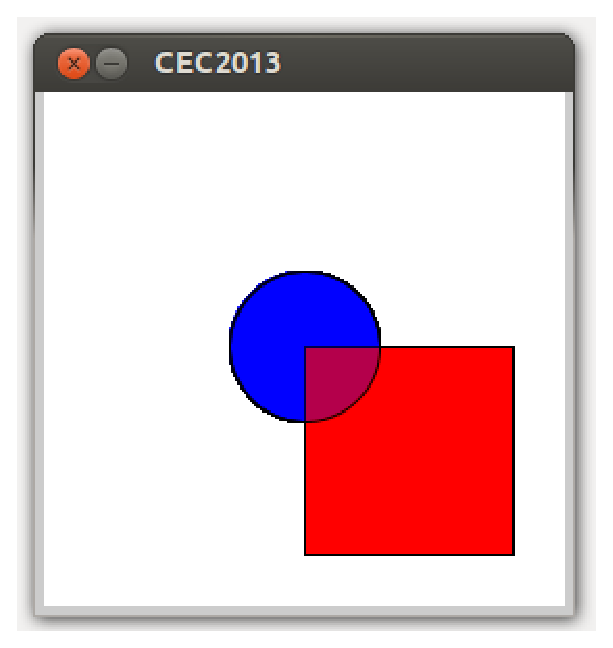
\includegraphics[scale =0.45] {images/run.eps}
   \label{fig:subsketch}
 }

\label{fig:ide}
\caption{Processing IDE and sketch execution. }
\end{figure*}

However, being a light framework, there exist some disadvantages:
\begin{itemize}
\item More complex applications require more programming skills.
\item The calculations of large computer images are a bit inefficient (although expert programmers can manage OpenGL at low level to fix this).
\end{itemize}

There exist a lot of interactive artistic projects made with Processing, examples are: BLABLABLABLA

Processing is composed by several modules:

\begin{itemize}
\item Structure: Includes typical programming functions as is the case of return, draw (), void, and everything related to the structure of the program.
\item Environment: Formed by the functions that handle the modeling of the window: cursor, width, height, background, for example.
\item Data: formed by the data types that make up the different program variables (int, char, float).
\item Control: Consisting in relations operators.
\item Shape: it is formed by all functions of the treatment of figures 3D and 2D.
\item Input: input interactivity features such as functions for the mouse, keyboard or files.
\item Output: output interactivity features such as write on the screen, save the image or serial control.
\item Transform: transformations such as rotations or translations.
\item Lights and Cameras: Functions for the treatment of the lights and cameras.
\item Color: Functions to handle color of the figures.
\item Image: Functions for loading images or textures.
\item Rendary: Functions for rendering images.
\item Typography: Functions for dealing with text.
\item Math: Functions for dealing with all mathematical functionality.
\end{itemize}

The Color module can be used to analyze images taking into account their histogram. The color histogram represents the frequency of occurrence of each color intensities present in the image, by accounting for such sharing pixels color intensity values.

The histogram is composed of different ranges or bins that represent a value or set of values ​​of color intensity. The color space is defined as a model representation with respect to color intensity values: RGB (Red, Green, Blue) and HSV (Hue, Saturation and Value).  The resolution of the various components is not uniform but used an increased number of bits for representing the hue component, which for the two remaining two bits being sufficient in the case of Value. Figure \ref{fig:histogram} shows the RGB histogram of the image in the Figure \ref{fig:flevopark}.

\begin{figure}
\centering
   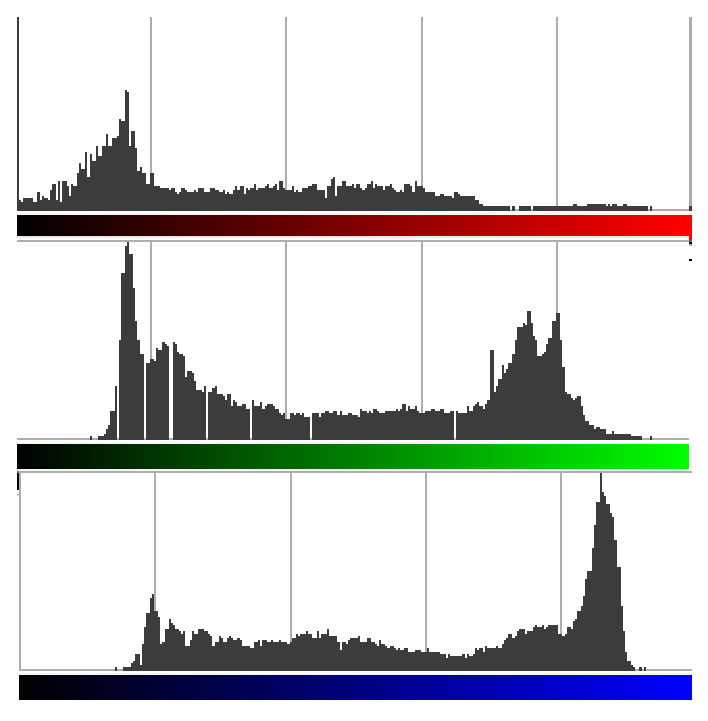
\includegraphics[scale =0.6] {images/histogram.eps}
\label{fig:histogram}
\caption{RGB histogram of the Figure \ref{fig:flevopark}. }
\end{figure}

\begin{figure}
\centering
   
\includegraphics[scale =3] {images/flevopark.eps}
\label{fig:flevopark}
\caption{Test image to compare with the Fitness functions of our algorithm.}
\end{figure}

\section{Experimental setup}

\subsection{Integrating Processing in Java}
Processing can be integrated with Java just adding a {\em jar} (a Java library) to existing software. The simplified code of the sketch (for example, the one shown in Figure \ref{sketch} is accessed extending the {\em PApplet} class. In this work, Processing has been integrated to an existent EA framework, OSGiLiath \cite{OSGILIATH}, a service-oriented framework based in Java that includes a lot of primitives and services for Evolutionary Computation. A new module called OSGiLiART has been added to the publicly-available source code of OSGiLiath (available in \url{http://www.osgiliath.org}) under a GPL License.

\subsection{Individual representation}

To test the Processing advantages and perform the experiments, the individual is a list of Processing Circles.

\subsection{Fitness used}
For this piece of research, we focused on two measures of aesthetics: basic histogram comparison and image matching. The fitness functions are included in the ``Error relative to Exemplars'' category, using Galanter \cite{galanter2012computational} classification.

%\subsubsection{Histogram comparision}\label{go:fitness:hist}
An histogram is a graphical representation of the tonal distribution in an image. The histogram for the property $i$ is computed following (\ref{eq:histogram}).


\begin{eqnarray}
	\label{eq:fitness}
	H(c, prop) = \frac{1}{N}\sum_{j=0}^N \left\{\begin{matrix}
1 & prop(j) = c\\ 
0 & otherwise
\end{matrix}\right. \\
	diff(h_1, h_2) = \sum_{j=0}^{255} |h_1(j) - h_2(j)| \\
	d_R(i) = diff(H(i, RED), H(target, RED))\\
	d_G(i) = diff(H(i, GREEN), H(target, GREEN))\\
	d_B(i) =  diff(H(i, BLUE), H(target, BLUE))\\
	fitness_{RGB}(i) = 1 - 128\frac{d_R(i) + d_G(i) + d_B(i)}{3} \\
	d_H(i) = diff(H(i, HUE), H(target, HUE))\\
	d_S(i) = diff(H(i, SAT), H(target, SAT))\\
	d_V(i) =  diff(H(i, VAL), H(target, VAL))\\
	fitness_{HSV}(i) = 1 - 128\frac{d_H(i) + d_S(i) + d_V(i)}{3}\\	
	fitness_{AVERAGE}(i) = \frac{fitness_{RGB}+fitness_{HSV}}{2}
\end{eqnarray}





\subsection{Parameters used}

A steady-state evolutionary algorithm has been used. Each individual is randomly generated at the initialization of the EA. The genome size is 50 elements (circles of maximum radium of 128 pixels). Population size has been set to 32 individuals. Crossover rate is 0.5, and a binary tournament has been selected for selection (that is, a pool of 16 parents is selected). Mutation probability is 0.04 (1/genomesize). Finally, the image size for eac individual is 256x256 pixels. The invidivuals have been compared with the histograms obtained from the image of Figure \ref{fig:flevopark}.

\section{Results} 
\label{sec:results}

Table \ref{tab:results} show the differences attained with each fitness used. As can be see... An example of evolution for each fitness can be see in Figure \ref{fig:rgbgens}, \ref{fig:hsvgens} and \ref{fig:averagegens}. 

\begin{table*}
\centering
\caption{Results for the different fitness. Only one histogram type is used, but the other values obtained are also added.}
\begin{tabular}{|c|c|c|c|} \hline
Differences used & Obtained RGB      		& Obtained HSV  & Obtained Average \\ \hline
RGB Histogram    & {\em 0.267 $\pm$ 0.012}	& 0.170 $\pm$ 0.010 	& 0.218 $\pm$ 0.009	\\ \hline
HSV Histogram    & 0.227 $\pm$ 0.017	& {\em 0.265 $\pm$ 0.021}	& 0.246 $\pm$ 0.010 \\ \hline
Average Histogram& 0.173 $\pm$ 0.012	& 0.294 $\pm$ 0.013	& {\em 0.234 $\pm$ 0.010} \\ \hline


\end{tabular}
\label{tab:results}
\end{table*}

\begin{figure}
   \includegraphics[angle=-90,scale =0.35] {images/rgbgens.eps}
\label{fig:rgbgens}
\caption{Evolution of the difference in RGB histogram of the best individual compared with the test image. }
\end{figure}

\begin{figure}
   \includegraphics[angle=-90,scale =0.35] {images/hsvgens.eps}
\label{fig:hsvgens}
\caption{Evolution of the difference in HSV histogram of the best individual compared with the test image. }
\end{figure}

\begin{figure}
   \includegraphics[angle=-90,scale =0.35] {images/averagegens.eps}
\label{fig:averagegens}
\caption{Evolution of the difference of average of RGB and HSV histogram of the best individual compared with the test image. }
\end{figure}

The best individuals attained are shown in Figure \ref{fig:bestinds}.

\begin{figure*}[ht]
\centering
\subfigure[Best individual using RGB]{
   
\includegraphics[scale =0.5] {images/RGB.eps}
   \label{fig:subfig2}
 }
\subfigure[Best individual using HSV]{
   
\includegraphics[scale =0.5] {images/HSV.eps}
   \label{fig:subfig1}
 }
\subfigure[Best individual using AVERAGE]{
   
\includegraphics[scale =0.5] {images/AVERAGE.eps}
   \label{fig:subfig2}
 }
\label{fig:bestinds}
\caption{Best individuals obtained with the three fitness used (HSV, RGB and AVERAGE). }
\end{figure*}


\section{Conclusions and Future Work}
\label{sec:conclusions}
This paper introduces an Evolutionary Algorithm that uses Processing to generate images and to extract image information. Individuals are represented as a list of Processing primitives and the fitness functions used are based in the similarity with an existent aesthetic image. Three different fitness function using histogram have been tested: difference with the HSV and RGB histograms, and an average difference of the two histograms at the same time.

The future work for this research work includes more experiment with other kind of individuals, appart from circles: using other primitives, such as rectangles or triangles, for example. With the use of textures and gradients would include a larger histogram EXTENDIDO. Finally, our intention is not create only static images, but use the Processing libraries to create evolutionary interactive art combining sounds and motion. A human guidance tool is also being developed to obtain human feedback to create a knowledge base for future experimentation.

The used software is Open Source and can be obtained in \url{http://www.osgiliath.org}.

\section*{acknowledgements}
This work has been supported in part by FPU research grant AP2009-2942 and projects EvOrq (TIC-3903), SINECA (0100DGT21285, Spanish Direccion General de Trafico) and TIN2011-28627-C04-02.

\bibliographystyle{IEEEtran}
\bibliography{evo_art}

\end{document}  
